\chapter{Experimental Results}\label{sec:results}
\begin{table}[t]
    \centering
    \ra{1.3}
    \resizebox{0.6\columnwidth}{!}{
    \begin{tabular}{@{}llcc@{}}\toprule
        Model & Dataset & $\text{ROC-AUC}_\text{TAG}$ & $\text{PR-AUC}_\text{TAG}$ \\ \midrule
        % \multicolumn{4}{c}{MTAT-Trained Experiments}\\\addlinespace
        Pons et al.$^\dagger$ & MTAT & \textbf{89.05} & 34.92 \\
        SampleCNN$^\dagger$ & MTAT & 88.56 & 34.38 \\
        CLMR (ours) & MTAT & 88.30 (\textit{88.86}) & \textit{34.60} (\textbf{35.0}) \\
        CPC (ours) & MTAT & 86.60 (87.99) & 30.98 (33.04) \\
        1D CNN$^\dagger$ & MTAT & 85.58 & 29.59 \\\midrule
        Pons et al.$^\dagger$ & MSD & 87.41 & \textbf{28.53} \\
        SampleCNN$^\dagger$ & MSD & \textbf{88.42} & - \\
        CLMR (ours) & MSD & 85.66 & 24.98 \\
        \bottomrule
        \end{tabular}
    }
    \caption{Tag prediction performance on the MagnaTagATune (MTAT) dataset, compared with fully supervised models$^\dagger$ trained on raw audio waveforms. The ROC-AUC and PR-AUC scores are tag-wise scores obtained by end-to-end training for the supervisd models. For the self-supervised models, the scores are obtained by training a \emph{linear}, logistic regression classifier on the MTAT dataset using the representations from self-supervised pre-training. Scores in parenthesis show performance when adding one hidden layer to the logistic regression classifier, making it a simple multi-layer perceptron.}
    \label{tab:magnatagatune_results}
\end{table}

\begin{table}[t]
    \centering
    \resizebox{0.8\columnwidth}{!}{
        \begin{tabular}{lllll}\toprule
        Temperature & $\text{ROC-AUC}_{\text{TAG}}$ & $\text{PR-AUC}_{\text{TAG}}$ & $\text{ROC-AUC}_{\text{CLIP}}$ & $\text{PR-AUC}_{\text{CLIP}}$ \\\midrule
        0.1         & 85.82                         & 30.33                        & 91.18                          & 64.10                         \\
        0.3         & 85.58                         & 30.35                        &                                &                               \\
        0.5         & 85.82                         & 30.49                        & 91.25                          & 64.78 \\                       
        \bottomrule
        \end{tabular}
    }
    \caption{Ablation study of the temperature parameter in the NT-Xent loss objective function.}
    \label{tab:temperature_ablation}
\end{table}

\begin{table}[t]
    \centering
    \resizebox{0.8\columnwidth}{!}{
        \begin{tabular}{lllll}\toprule
        Sample rate & $\text{ROC-AUC}_{\text{TAG}}$ & $\text{PR-AUC}_{\text{TAG}}$ & $\text{ROC-AUC}_{\text{CLIP}}$ & $\text{PR-AUC}_{\text{CLIP}}$ \\\midrule
        8000 & 84.78 & 29.77 & 90.60 & 62.94 \\
        16000 & 85.46 & 30.42 & 90.97 & 64.08 \\
        22050 & 85.82 & 30.49 & 91.25 & 64.78 \\                       
        \bottomrule
        \end{tabular}
    }
    \caption{Effect of the sample rate on tag prediction performance.}
    \label{tab:temperature_ablation}
\end{table}

\begin{figure}[t]
    \centering
    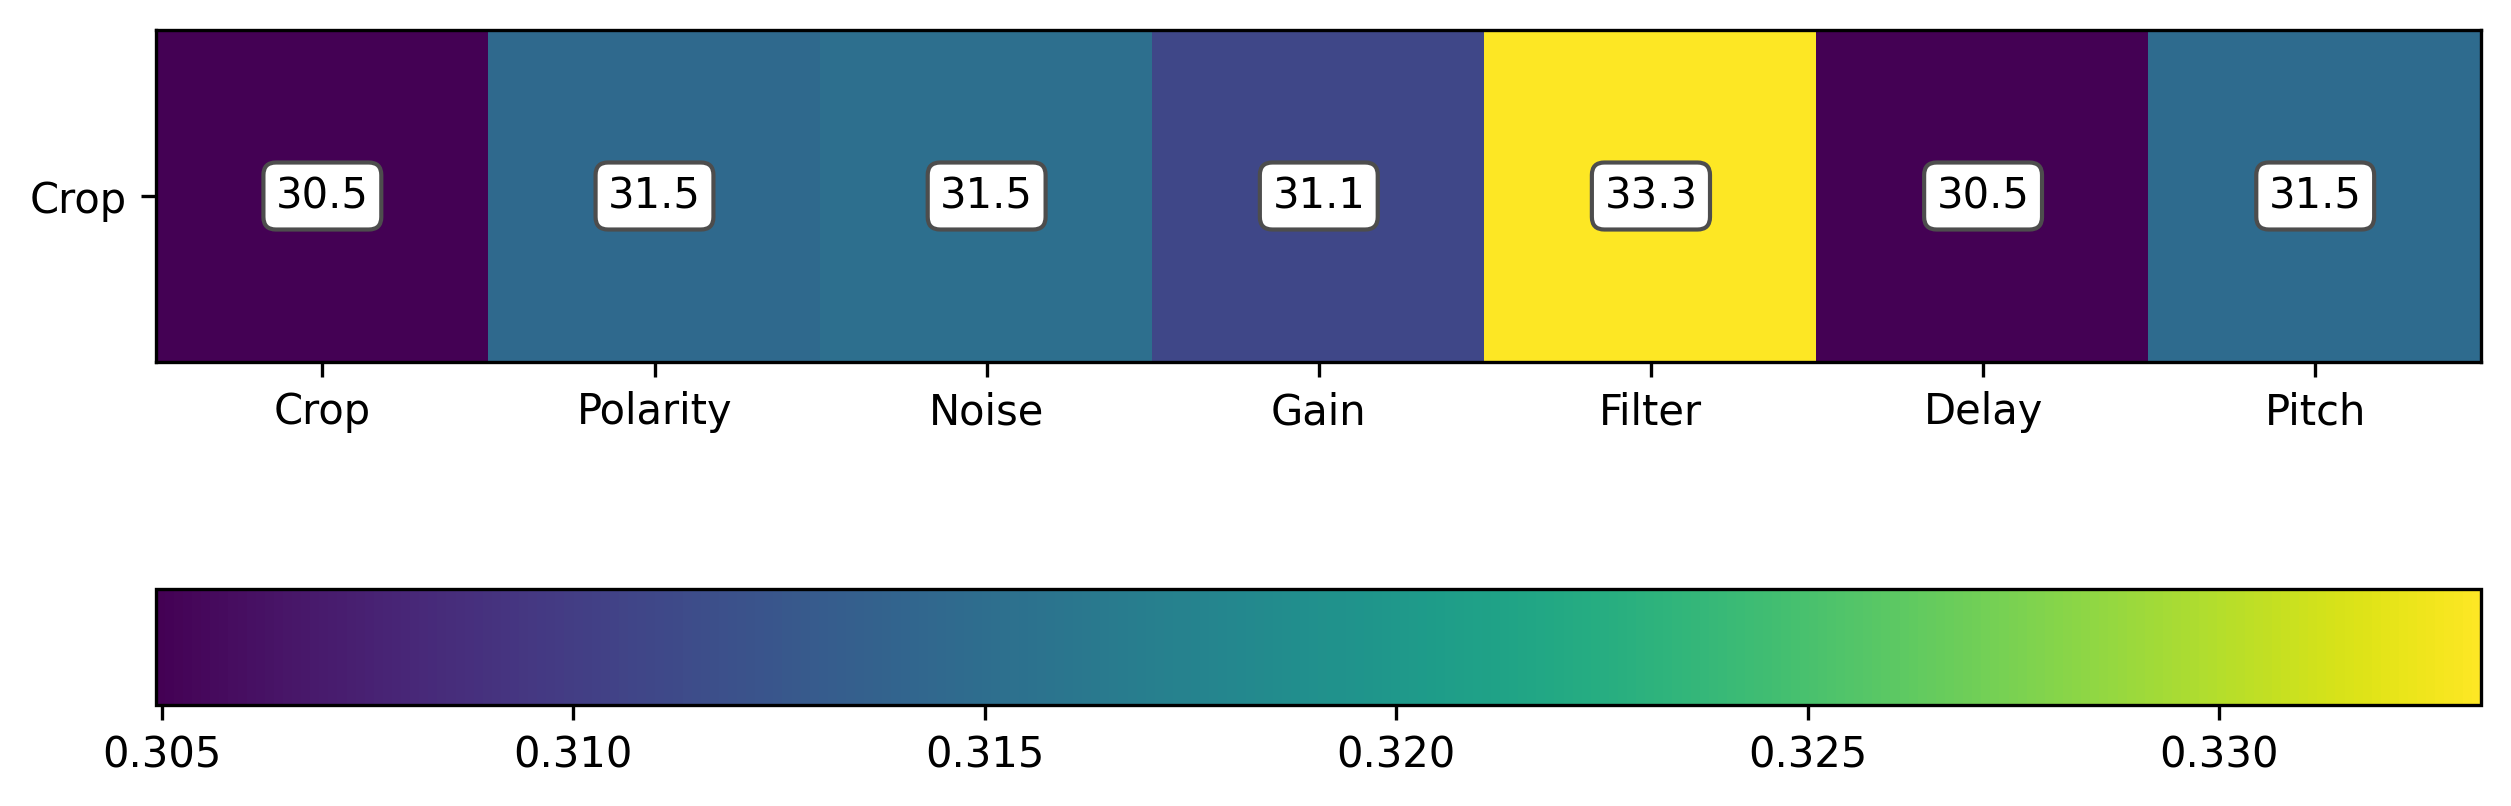
\includegraphics[width=\columnwidth]{figs/transformation_study.png}
    \caption{Transformation study}
    \label{fig:transformation_study}
\end{figure}

\begin{figure}[t]
    \centering
    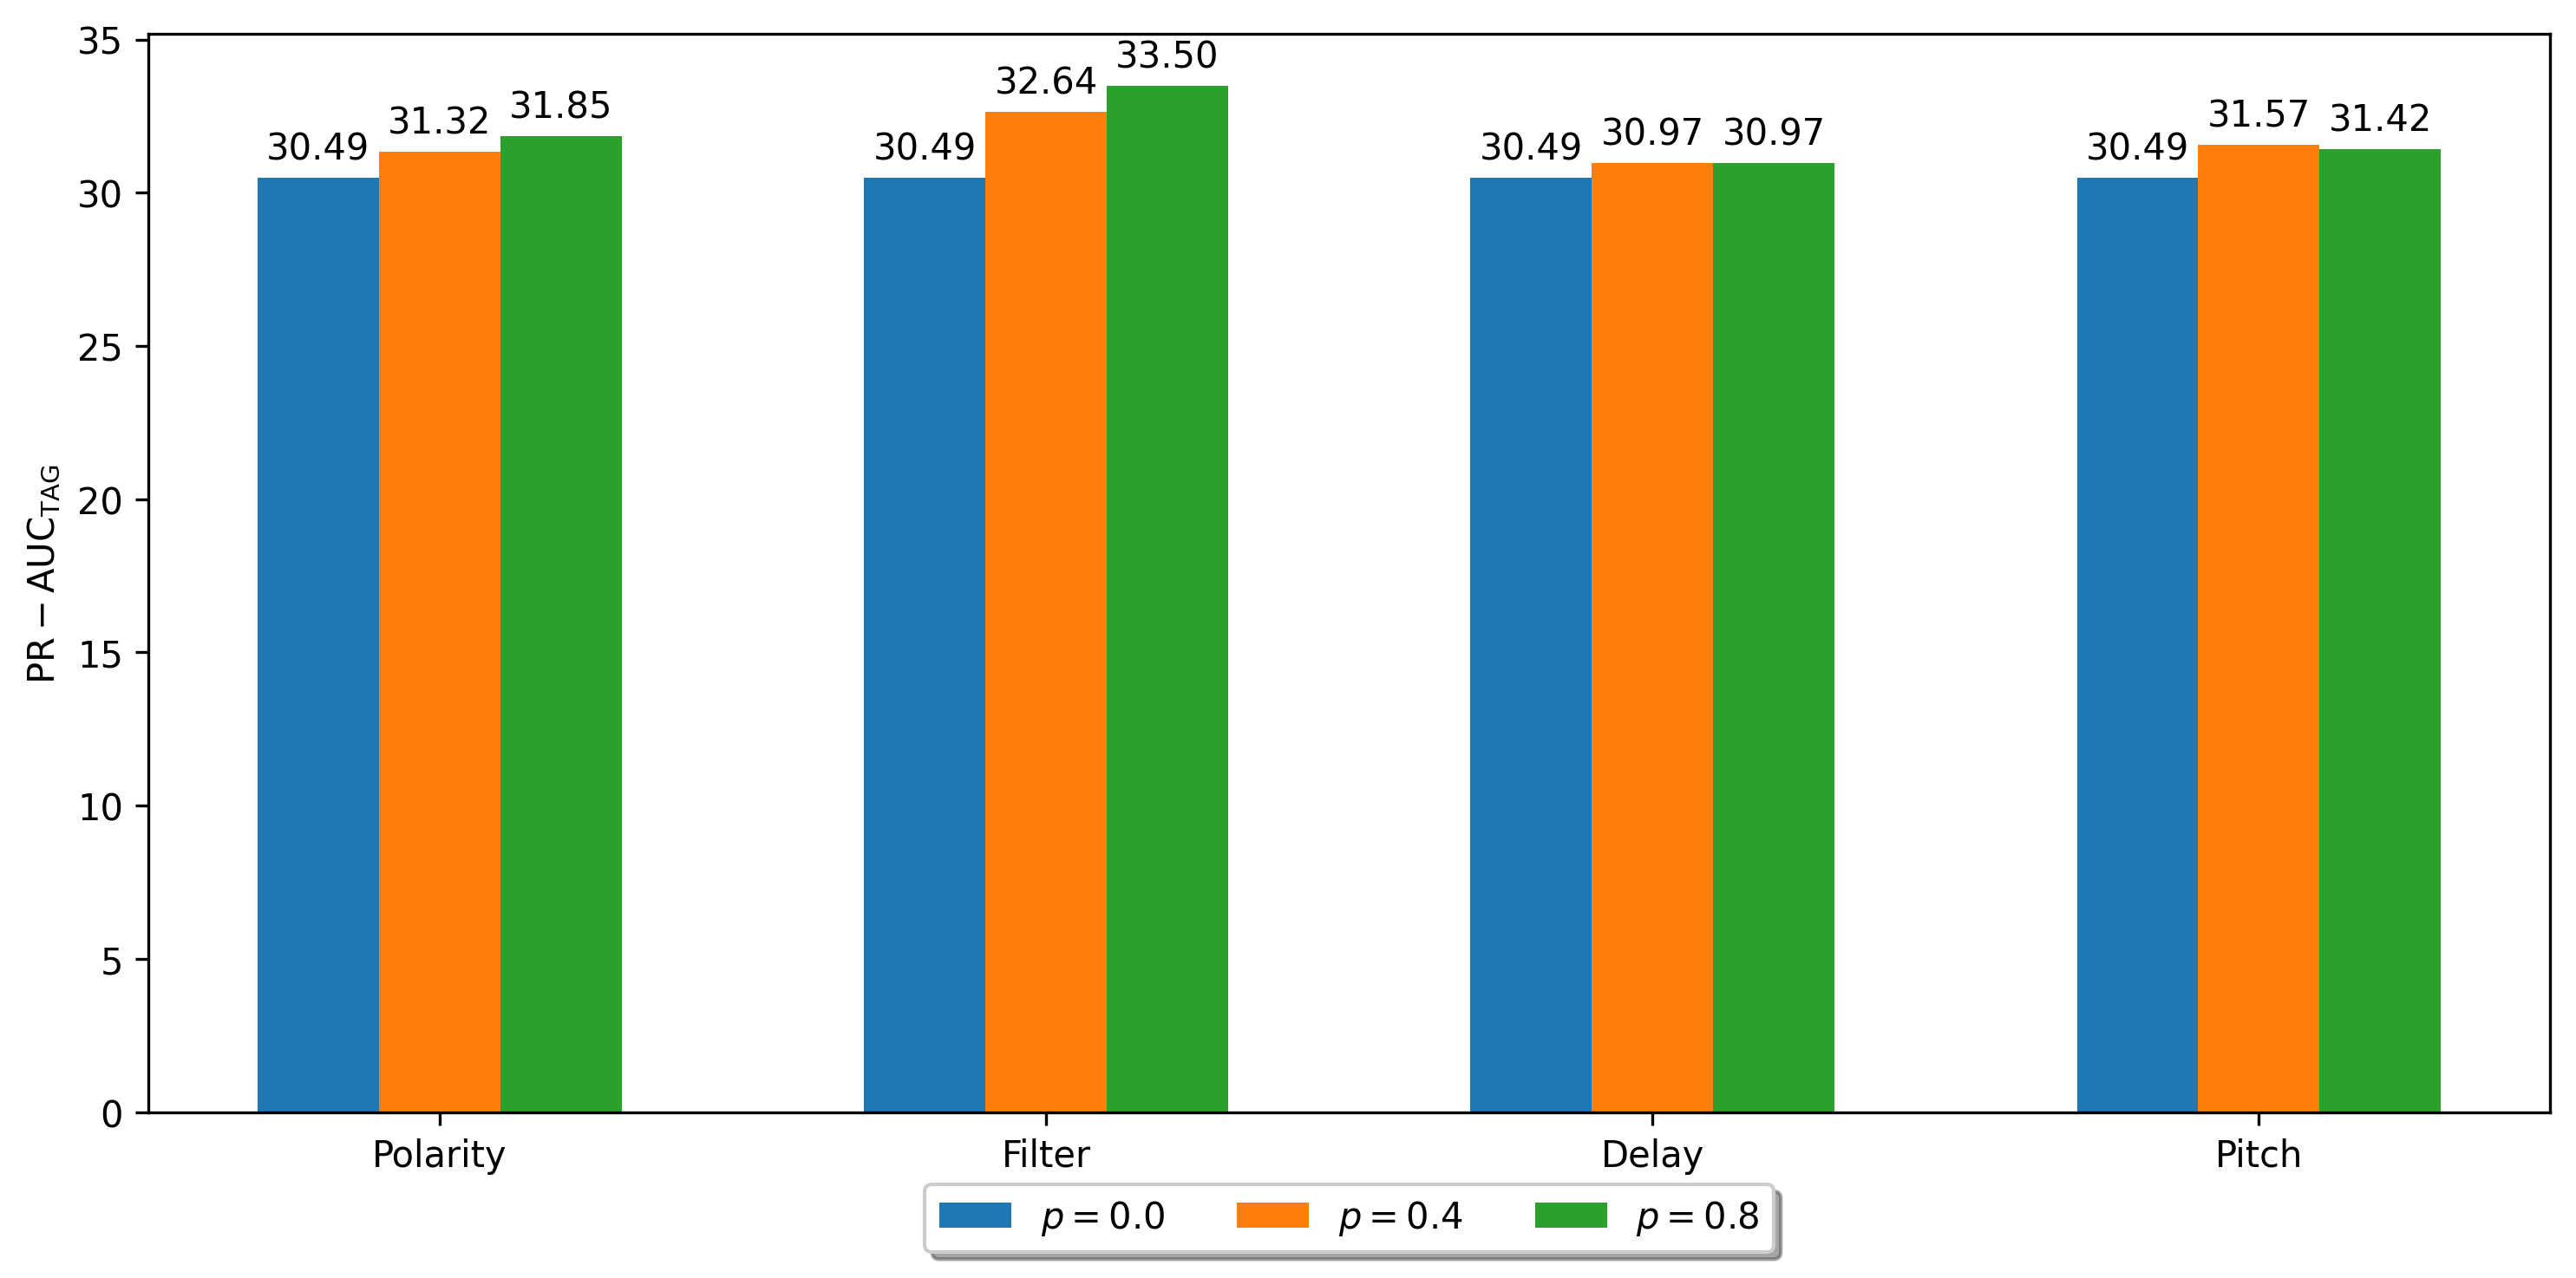
\includegraphics[width=\columnwidth]{figs/transformation_probabilities.png}
    \caption{Transformation study}
    \label{fig:transformation_probabilities}
\end{figure}





\section{Quantitative and Qualitative Evaluation}
The evaluation metrics for the best-performing models are shown in Table \ref{tab:magnatagatune_results}. Both CPC and CLMR show competitive performance with fully supervised models in the music classification task, despite being pre-trained without ground truth and using a simple, linear classifier for evaluation. A non-linear projector network positively impacts the performance of the model. Adding only one extra hidden layer to the classifier increases the results by $4\%$, making the gap between supervised end-to-end baselines even smaller.
% It is clear from these results that useful representations can be learned from high-dimensional signals of raw audio even without access to ground truth labels. 

For a qualitative view of the representations, we show how cleanly they are  separable using a $t$-SNE manifold in Figure \ref{fig:tsne_manifold}. Figure \ref{fig:tag_scores} shows in more detail that the difference in performance between self-supervised and supervised models is marginal: there is no single tag performance difference larger than 4\% ROC-AUC, and for practical purposes, CLMR and CPC retrieve tags practically identically to supervised models.

\begin{figure}[t]
    \centering
    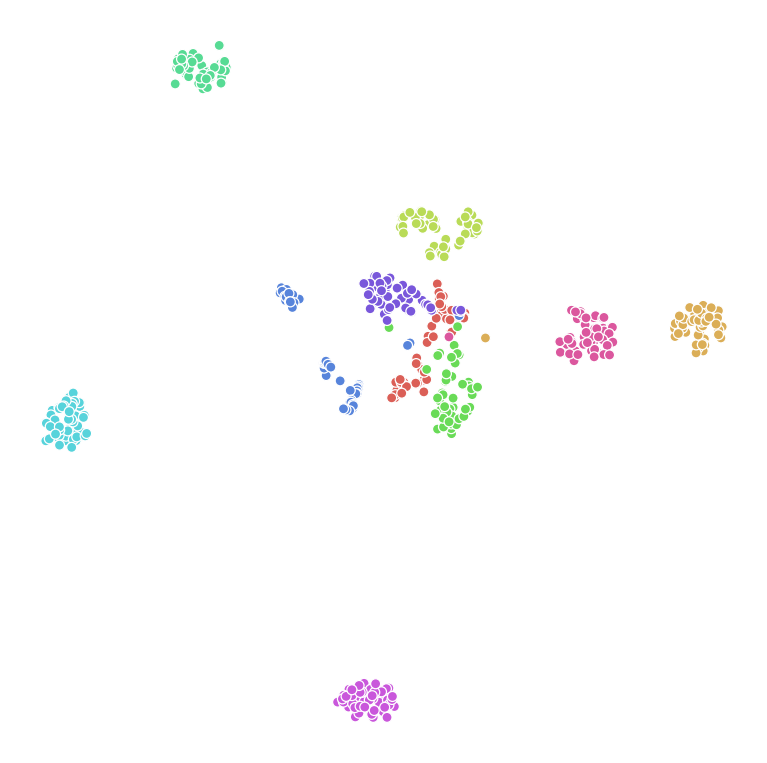
\includegraphics[width=0.75\columnwidth]{figs/tsne-clmr.png}
    \caption{$t$-SNE manifold visualisation from audio representations learned by a converged CLMR model of a subset of 10 tracks with each 60 segments. Every color represents a unique track.}
    \label{fig:tsne_manifold}
\end{figure}



\section{Data Augmentations and Mini-Batch Size}
Our results show that all data augmentations, with the exception of adding random noise, contribute to a higher accuracy score. Using $p_{\mathrm{filter}}=0.4$ increases PR-AUC by $5.5\%$, and the performance difference is $8\%$ when all augmentations are done instead of only random trimming. When re-sampling the audio to 8\,000~Hz and 12\,000~Hz respectively, there is a marginal penalty to the final accuracy scores for the self-supervised models, which is in line with previous work\cite{lee2018samplecnn}. Increasing the batch size to 192 and 128 respectively also increases final evaluation scores. We refer the reader to the supplementary material for a complete overview of the results obtained with different augmentation and model parameters.

\subsection{Transfer Learning}
The results of the transfer learning experiments are shown in Table \ref{tab:magnatagatune_results}. Both CPC and CLMR show the ability to learn effective representations from datasets different from the evaluation dataset without ground truth, and even exceed accuracy scores of previous, supervised end-to-end systems on raw audio\cite{dieleman2014end}. Moreover, both models demonstrate the ability to learn useful representations on small datasets like GTZAN. The CLMR model performs better when pre-trained on larger datasets, which is expected as it heavily relies on the number of unique, independent examples to create correlated augmentations. When pre-training on smaller datasets, the autoregressive modelling in CPC can find more useful representations for downstream tasks.
%contribute to more useful representations for downstream tasks.

\begin{table}[t]
    \centering
    \ra{1.3}
    \resizebox{\columnwidth}{!}{
    \begin{tabular}{@{}lllcc@{}}\toprule
        Model & Train Dataset & Eval. Dataset &  ROC-AUC & PR-AUC \\ \midrule
        CLMR & MSD & MTAT &  \textbf{86.57} & \textbf{32.04} \\
        CPC & FMA & MTAT & 86.34 (\underline{87.79}) & 30.71 (\underline{32.47}) \\
        CLMR & FMA & MTAT & 86.22 (86.63) & 30.58 (31.22) \\
        CPC & Billboard & MTAT & 85.78 (86.25) & 29.68 (30.15) \\
        CPC & GTZAN & MTAT & 83.44 (86.06) & 26.88 (29.72) \\
        CLMR & Billboard & MTAT & 82.73 (84.22) & 26.86 (27.82) \\
        CLMR & GTZAN & MTAT & 81.88 (85.43) & 26.18 (29.49) \\
        \bottomrule
        \end{tabular}
    }
    \caption{Performance of the self-supervised models when pre-trained on datasets different from the evaluation dataset, again using a linear classifier to evaluate.}
    \label{tab:magnatagatune_results}
\end{table}



\section{Visualising filters}
Figure \ref{fig:filter_visualisation} shows the magnitude spectrum of the learned filters of the sample-level convolutional layers (layers 1, 4 and 6) for CLMR and CPC, pre-trained on the MTAT and Billboard dataset. In CLMR, the first layer is sensitive to a single, very small band of frequencies around 7500~Hz, while in higher layers, the filters spread themselves first linearly and then non-linearly across the full range. CPC shows a similar pattern in the lowest layer, but shows a strong activation of two frequencies that span an octave. Interestingly, CLMR shows a similar filter structure for the Billboard data set as fully supervised models that were trained on the MTAT dataset \cite{dieleman2014end,lee2018samplecnn}. The Billboard dataset is significantly less diverse in genre, suggesting the self-supervised model focuses more on such frequency-band related differences than it does for the more diverse Magna\-Tag\-A\-Tune.

